\section{Event selection}
\label{sec:htoinv_event_selection}

The event selection aims to strike a balance between rejecting as many background events while retaining as much signal as possible. The preselection, in Chpt.~\ref{subsec:htoinv_preselection}, is applied to data and simulation in all analysis regions and categories to do just that. Filters to reject potentially-mismeasured events and those that lead to incorrect \ptvecmiss calculations are documented in Chpt.~\ref{subsec:htoinv_other_filters}. A strategy to combat the HEM issue faced in 2018 (detailed in Chpt.~\ref{subsec:htoinv_data}) is given in Chpt.~\ref{subsec:htoinv_hem_mitigation}.


%=========================================================


\subsection{Preselection}
\label{subsec:htoinv_preselection}

The preselection is designed to discriminate between signal and background events, and is characterised by applying the following cuts:

\medskip % medium skip to nicely separate the start (end) of the list with the end (start) of the previous (next) paragraph (ignored if the space would occur at the top of a new page). Should be 9 pt (i.e., half a line since I use 12 pt text and 1.5 line spacing)
\begin{easylist}[itemize]
    \cutflowlistprops
    & $\ptjone > \text{80} \GeV$
    & $\HT > \text{200} \GeV$
    & $\mht > \text{200} \GeV$
    & $\ptmiss > \text{200} \GeV$
    & $\mht/\ptmiss > \text{0.8}$
    & $\mht/\ptmiss < \text{1.2}$
    & $n_{\vlooseTau} = \text{0}$
\end{easylist}

\medskip
% No indent so it doesn't look weird just after the hanging list
\noindent{}To ensure orthogonality with the phase space occupied by the \acrshort{vbf} topology, the two leading \glspl{jet} must be within the acceptance of the tracker, and events must fail one or more of the following criteria:
\medskip
\begin{easylist}[itemize]
    \cutflowlistprops
    & $\ptjtwo > \text{40}\GeV$
    & $\etajone \cdot \etajtwo < \text{0}$
    & $\ptmiss \geq \text{250}\GeV$
    & $\abs{\Delta \eta(\jone, \, \jtwo)} > \text{1.0}$
    & $\mjj > \text{200}\GeV$
    & $\Delta \phi(\jone, \, \jtwo) < \text{1.5}$
\end{easylist}


%=========================================================


\subsection{Additional filters}
\label{subsec:htoinv_other_filters}

Further selections are applied to filter poorly measured or mis-reconstructed events in both data and \acrshort{mc}. These are applied to all years, regions, and categories unless stated otherwise.

A ``muon \gls{jet} filter'' rejects events with mis-reconstructed muons by requiring all \glspl{jet} with $\pt > \text{200}\GeV$ to have a muon energy fraction $f_{\mathrm{E}}^{\Pmu} < \text{0.5}$ or $\Delta\phi(\mathrm{j}, \, \ptvecmiss) < \pi - \text{0.4}$.

Events containing a \gls{jet} in the forward region with $\pt > \text{50}\GeV$ are rejected since they are more susceptible to mismeasurement in that area of the detector. An additional benefit is the further separation of signal from background.

Charged ($f_{\mathrm{E}}^{h\pm}$) and neutral hadron energy fraction ($f_{\mathrm{E}}^{h0}$) requirements are applied to all \glspl{jet} via fulfillment of the tight \gls{jet} ID criteria (see Chpt.~\ref{subsec:objects_jets}). Furthermore, stricter selections are placed on the leading two \glspl{jet} as follows:

\medskip

\begin{easylist}[itemize]
    \cutflowlistprops
    & $f_{\mathrm{E}}^{h\pm}(\jone) > \text{0.1}$
    & $f_{\mathrm{E}}^{h0}(\jone) < \text{0.8}$
    & $f_{\mathrm{E}}^{h\pm}(\jtwo) > \text{0.1}$
    & $f_{\mathrm{E}}^{h0}(\jtwo) < \text{0.8}$
\end{easylist}

\medskip

\noindent{}In the \acrshort{qcd} \glspl{SB}, despite the requirement of $\ptmiss > \text{200}\GeV$, an excess in data was observed for events with low missing transverse momentum calculated from track momenta ($\ptmissTrk$). This indicated a significant presence of neutral particles in such events, warranting a cut of $\ptmissTrk > \text{80}\GeV$ in the signal region and \glspl{SB}.

A discrepancy between the directions of the \htvecmiss and \ptvecmiss were found to be present in both the \ttH and \VH categories, prompting the requirement $\Delta\phi(\htvecmiss, \, \ptvecmiss) < \text{0.5}$ everywhere. In the \ttH categories, this was further tightened. Large differences between the azimuthal angle of the missing transverse momentum calculated with \acrlong{pf} (\ptvecmiss), and either from track momenta (\ptvecmissTrk) or \glspl{jet} (\htvecmiss) are indicative of an inconsistent event description. An elliptical cut is therefore placed in the plane of $\Delta\phi(\ptvecmiss, \, \ptvecmissTrk)$ and $\Delta\phi(\htvecmiss, \, \ptvecmiss)$ for events in the signal region and sidebands for \ttH:
\begin{equation}
    \sqrt{ \Delta\phi(\ptvecmiss, \, \ptvecmissTrk)^2 + 4 \cdot \Delta\phi(\htvecmiss, \, \ptvecmiss)^2 } < 1.0
\end{equation}
The filters described below were recommended by the MET \acrshort{pog}~\cite{cmsmetfilterspage} to remove events with potentially miscalculated \ptvecmiss:
\medskip
\begin{easylist}[itemize]
    \easylistprops
    & Primary vertex filter to remove events failing vertex quality criteria
    & Beam halo filter
    & \acrshort{hcal} barrel and end cap noise filters
    & Filter for dead cells in the \acrshort{ecal} when constructing trigger primitives
    & Filter for low-quality \acrlong{pf} muons
\end{easylist}

\medskip

\noindent{}There are supplementary filters applied only to data. These are to generally mitigate \acrshort{ecal} end cap supercrystal noise, as well as crystals where losses of transparency would otherwise require large laser corrections.


%=========================================================


\subsection{Mitigating the HEM issue}
\label{subsec:htoinv_hem_mitigation}

During the 2018 data taking period, the HEM issue forced additional measures to be taken that suppressed its effect on the events. For the data recorded within affected period, region-dependent selections were updated to remove events that met the following criteria:
\medskip
\begin{easylist}[itemize]
    \cutflowlistprops
    & $-\text{1.8} < \phi(\ptvecmiss) < -\text{0.6}$ in the signal region and \glspl{SB}
    & Any veto electron \vetoEle with $\pt > \text{10}\GeV$, $-\text{3.0} < \eta < -\text{1.4}$, and $-\text{1.57} < \phi < -\text{0.87}$ in the \singleEleCr and \doubleEleCr \glspl{CR}
\end{easylist}

\medskip

\noindent{}Events in simulation that met the same criteria were instead weighted by the integrated luminosity from 2018 that was not affected by the issue (i.e., 21.1\fbinv) rather than the entire year. It is applicable under the assumption that both data and simulation are distributed comparably in the $\eta$-$\phi$ portions of the detector when the issue was not present. Given geometric variables agree very well between data and simulation in the analysis, and corrections are implemented to further synchronise them, the assumption is valid.

The effect of the HEM issue can be seen in Fig.~\ref{fig:htoinv_hem_issue_met_phi}. The $\phi(\ptvecmiss)$ distribution is shown in a \gls{SB} to the signal region defined by inverting the \omegaTilde variable (see Chpt.~\ref{subsubsec:htoinv_ang_var_optimisation}) since it kinematically resembles the signal region, and the data--simulation discrepancy can be removed while still blind to the data in the signal region.

\begin{figure}[htbp]
    \centering
    \begin{subfigure}[b]{0.4\textwidth}
        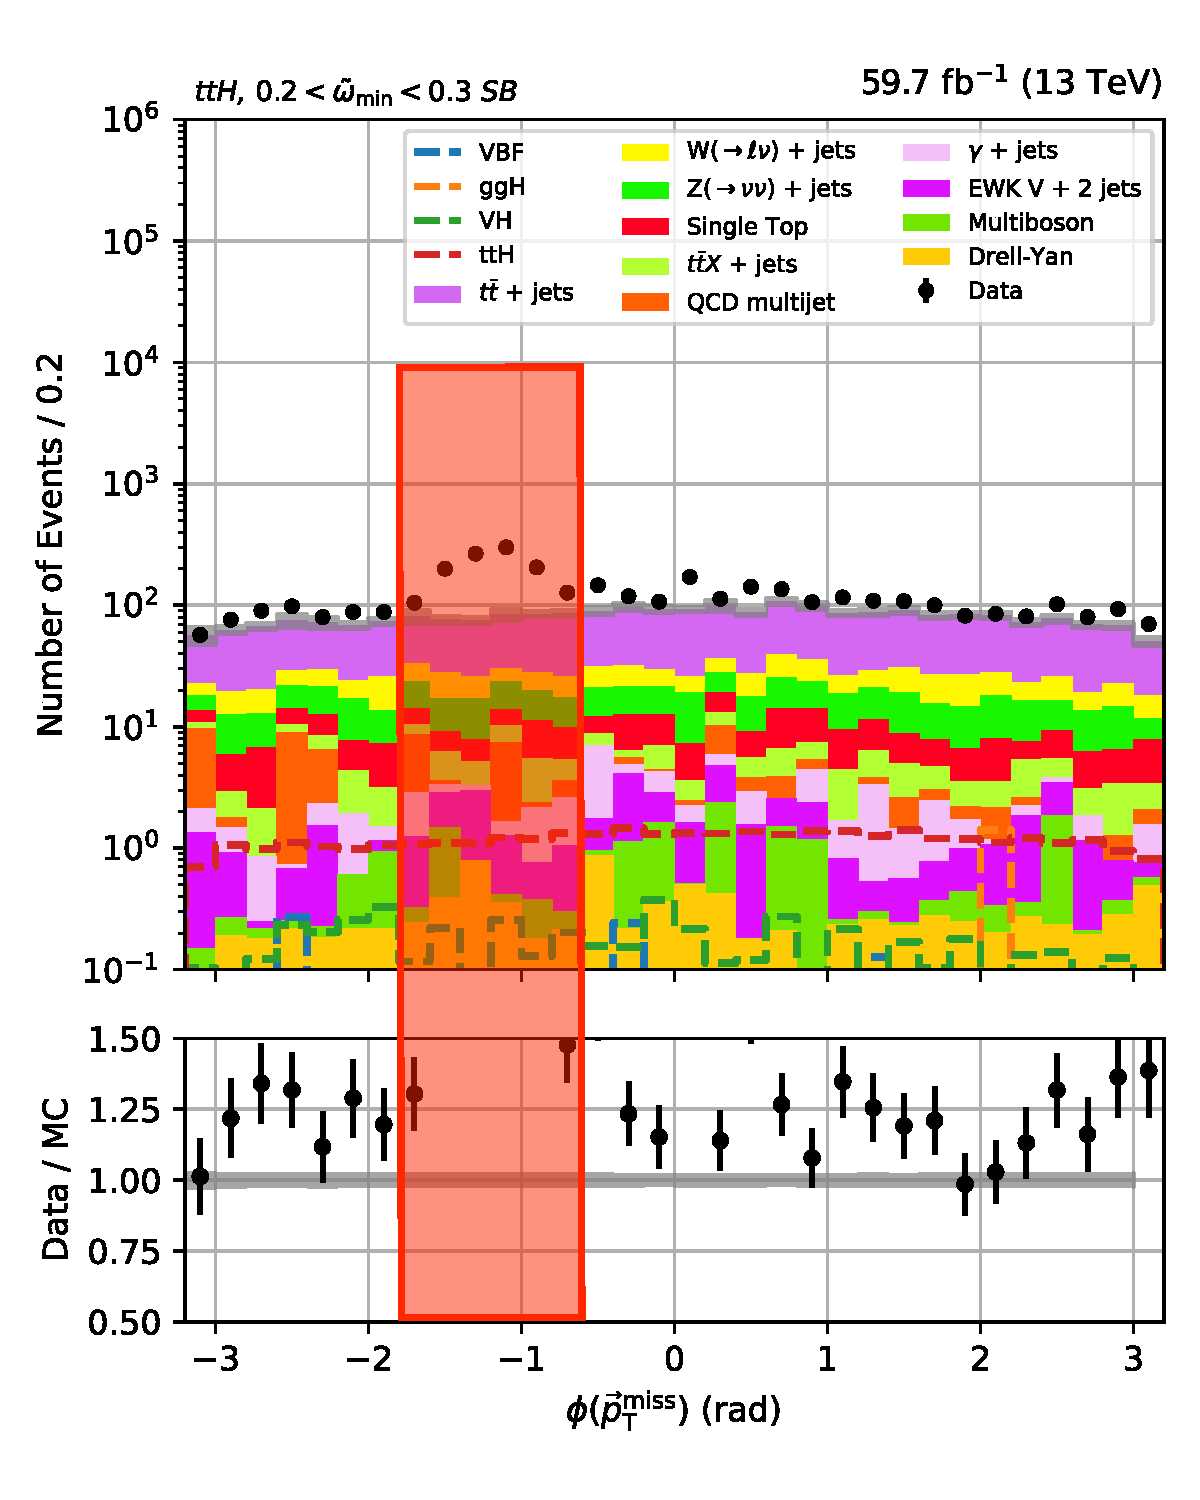
\includegraphics[width=\textwidth]{figures/hem_issue/sideband_4/met_phi/met_phi_ttH_before_annotated.pdf}
        \caption{\ttH inclusive category}
    \end{subfigure}
    \hspace{0.1\textwidth}
    \begin{subfigure}[b]{0.4\textwidth}
        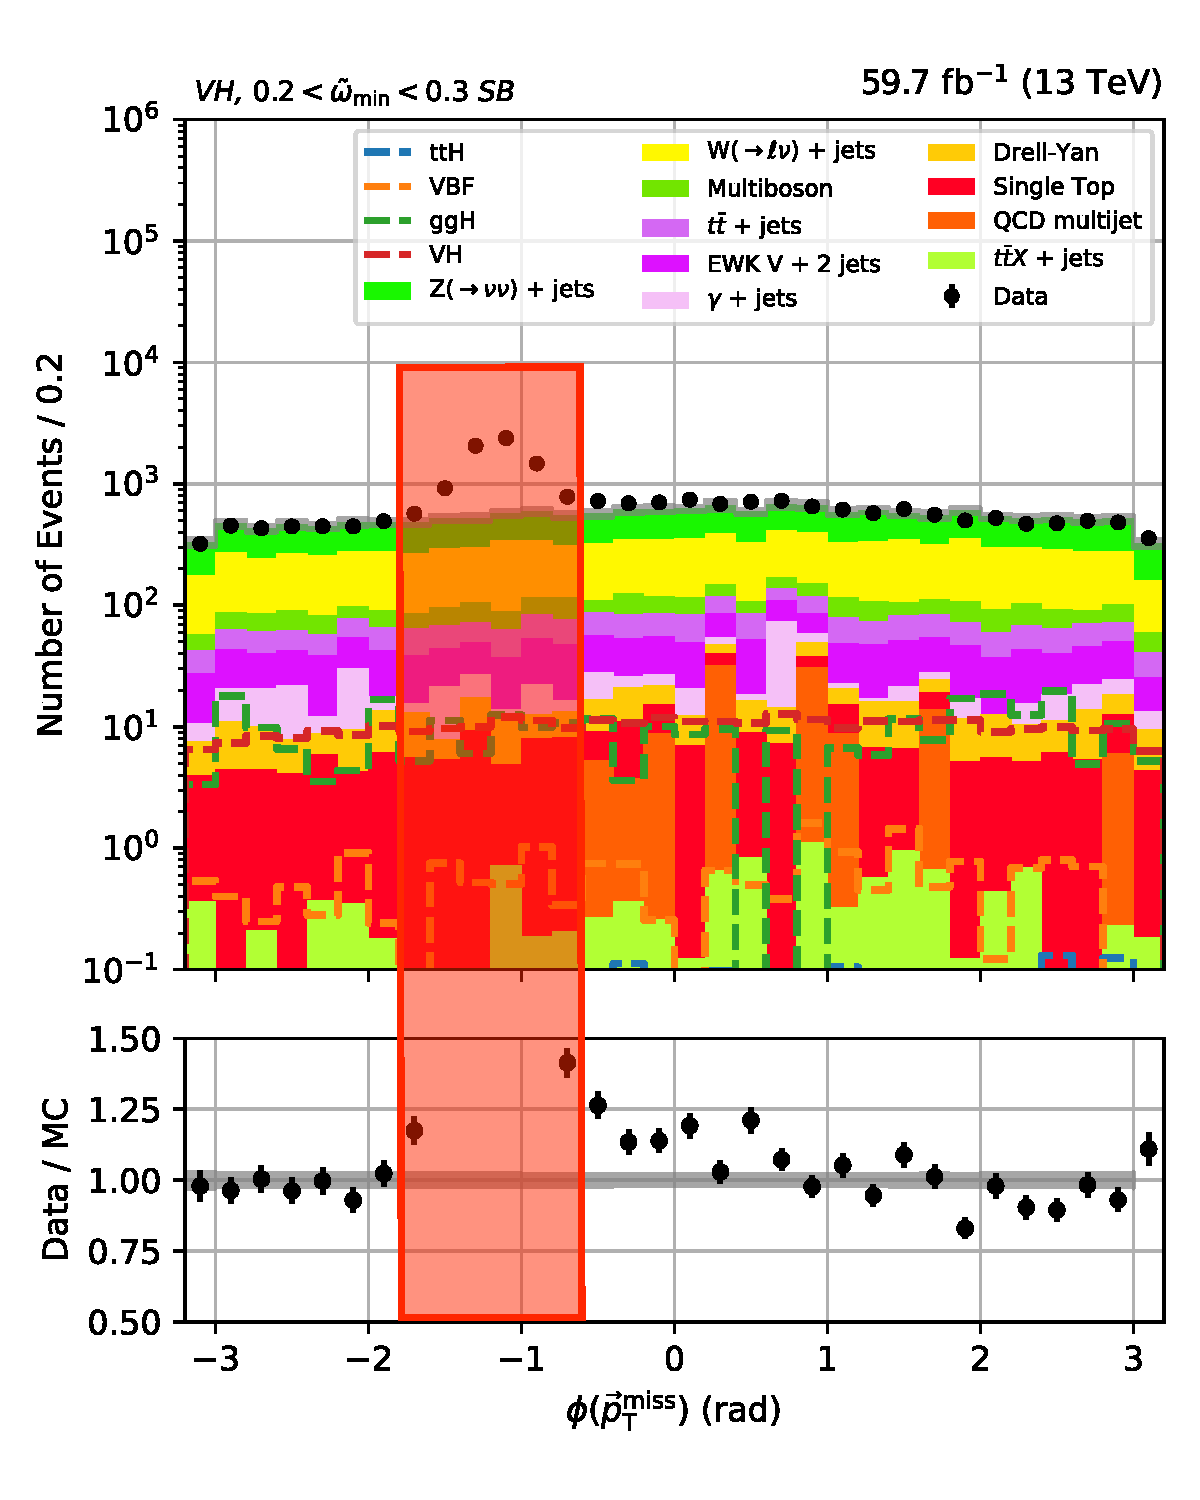
\includegraphics[width=\textwidth]{figures/hem_issue/sideband_4/met_phi/met_phi_VH_before_annotated.pdf}
        \caption{\VH inclusive category}
    \end{subfigure}
    \caption[The azimuthal angle of the \ptvecmiss inclusive in the \ttH and \VH categories before applying the selections designed to mitigate the HEM issue in 2018]{The azimuthal angle of the \ptvecmiss inclusive in the \ttH and \VH categories before applying the selections designed to mitigate the HEM issue in 2018. The loose \omegaTilde \gls{SB} is used to demonstrate the effect. A red box encloses the sector that is removed by the selection applied in the signal region and \glspl{SB}.}
    \label{fig:htoinv_hem_issue_met_phi}
\end{figure}
